\chapter{Program}

\section{V čem psát program a jeho tvorba}

Program jsem se rozhodla psát v programu vizual studio code. Pracovala jsem s ním v minulosti a i zde platilo, že jsem kolem měla lidi, který by mi mohli pomoct ve chvíli, když bych měla s něčím problém. Pro psaní kódu jsem použila školní knihovny na programovaná LED světel, které byli původně vyrobeny pro letní robotický tábor a tak jsem měla o něco lehčí práci, protože jsem knihovny nemusela vytvářet sama.  
Na programování jsou použila pevný LED pásek.

\begin{figure}[htbp]
	\centering
	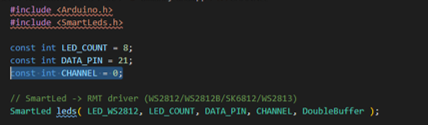
\includegraphics[width=0.65\textwidth]{img/015 img/zacatek-programu.png}
	\caption{Začátek programu}
%	\label{fig:install-sdk-1}
\end{figure}

První dva řádky jsou knihovny, které jsem při psaní využívala. Další tři jsou definované proměnné, které určují, kolik LED světel pásek má (8), jaký pin zajišťuje komunikaci s ESP32-DevKit (21), a číslo, které určuje, jaké číslo ponese první LED světlo s tím,  že další LEDky byli očíslovány chronilogicky.

\newpage

\section{První mód světla}
Jako první barvu prvního módu jsem rozhodla že bude červená. jen obyčejná červená bez jakýkoliv jiných barev nebo blikání. Nejdříve jsem ale musela nadefinvat funkci, která mi pomohla v dalším postupu a usnadnila mi manipulaci se všemi LEDkami. 

    \begin{figure}[htbp]
	\centering
	\begin{minipage}[b]{0.5\textwidth}
		\centering
		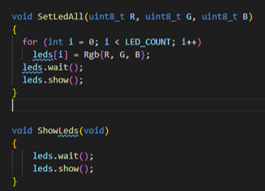
\includegraphics[width=0.75\textwidth]{img/015 img/definovane-funkce.png}
		\caption{Funkce}
%		\label{fig:gear-sketch1}
	\end{minipage}
	\qquad
	\begin{minipage}[b]{0.4\textwidth}
		\centering
		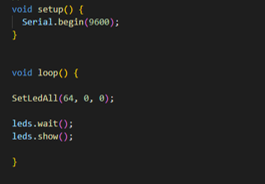
\includegraphics[width=1\textwidth]{img/015 img/Program1-červená.png}
		\caption{Program}
%		\label{fig:gear-sketch2}
	\end{minipage}
\end{figure}

Nejdříve jsem si nadefinovala funkci SetLEDAll, která mi při použití určitého příkazu, jak se LED-ky mají rozsvítit, aplikovala tento příkaz na všechny LED-ky na pásku, a umožnila mi jednodušší manipulaci s programem v pozdější fázy, když jsem všechny tyto módy přepisovala do jednoho programu. 
%Funkce ShowLeds v sobě zase obsahovala dva příkazy, které se v programu nacházeli pro stabilizaci LEDek. 
Na dalším obrázku je ukázán samotný program, který provedl to, že zavolal finkci, že se má daná barva aplikovat na všechny LED-ky a nastavila je na tlumeně červenou barvu. Tluměně červenou proto, že LEDky zářili opravdu intenzivně a při jasu na 255 mě z nich začali bolet oči. Proto jsem jas červené nechala na pouhé štvrtině toho, co by LEDky zvládly.

\section{Druhý mód světla}
%nechci aby to blikalo jako blázen 
Jako druhý mód světla jsem se rozhodla, že použiju světle modrou barvu, která se bude pomalu stupňovat a pak tlumit a vznikne efekt pulzujícího modrého světla. Tohodle jsem docílila pomocí programu: 

\begin{figure}[htbp]
	\centering
	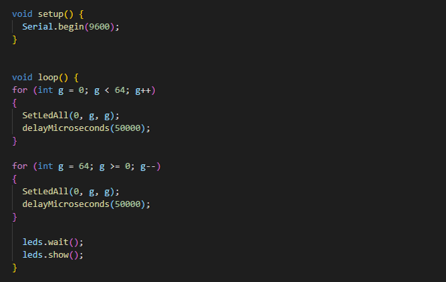
\includegraphics[width=0.57\textwidth]{img/015 img/program2-Ledova-ruze.png}
	\caption{Program č. 2}
%	\label{fig:install-sdk-3}
\end{figure}


Tento program Je navrhnut tak, že se zhasnuté LEDky začnou pomalu rozsvěcovat do jasné modré a poté znovu zhasínat do naprosté tmy. A jelikož byl tento příkaz napsán v části loop, tento cyklus se bude opakovat do té doby, dokud nebude zavolána jiná funkce, nebo nebude ESP32-Devkit odpojen. Docílí se tak moc pěkného pulzujícího modrého efektu. Opět zde není použita plná síla LED světel, aby byly šetřeny moje oči.  


\section{Třetí mód světla}
Jelikož mi Nápad na to, jak jsem udělala pomalu pulzující světlo, skvělý. Rozhodla jsem se něco podobného aplikovat i na třetí mód. Tentokrát jsem ale skusila, jaké by to bylo, kdyby červená barva pomalu přešla do žluté a ze žluté do zelené a pak zase zpět. 

\begin{figure}[htbp]
	\centering
	\includegraphics[width=0.5\textwidth]{img/015 img/program3-oheň.png}
	\caption{Program č. 2}
	%	\label{fig:install-sdk-3}
\end{figure}

Program na tenhle mód je hodně jednoduchý a využívá podobného principu jako ten předchozí. Opět tu je spoždění, aby světlo bláznivě neblikalo. Původně jsem chtěla aby barva připomínala oheň,což mi moc nevyšlo ale i tak to je moc pěkný přechod barvy, který při umístění do plastového krystalu nebo růže (něco jako žárovky) vytvoří nádherný efekt.


\section{Čtvrtý mód světla}
Původně jsem nechtěla mít víc, než tři mmódy na mých LEDkých, ale neodolala jsem vidině, že budu mít mód který mi zařítí, že barevný přechod bude procházet celým barevných spektrem  dokola a dokola. 

%nevím co s tímto obrázkem. Jak udělat aby šel text hned vedle obrázku? 
\begin{figure}[htbp]
	\centering
	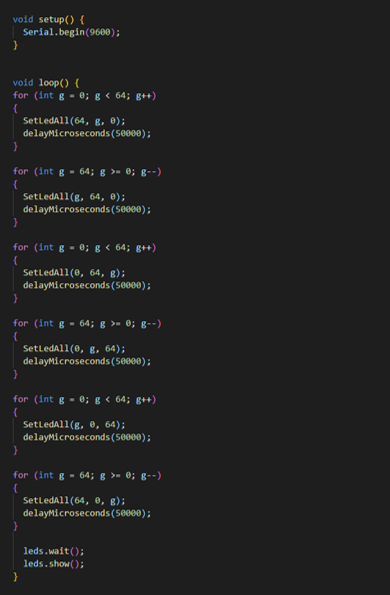
\includegraphics[width=0.5\textwidth]{img/015 img/program4-duha.png}
	\caption{Program č. 2}
	%	\label{fig:install-sdk-3}
\end{figure}

V podstatě na tomto programu není vůbec nic nového. Zase začíná na červené, kdy pomalu projde přež žlutou k zelené, dále pokračuje na světle modrou a tmavě modrou, až se dostane z fialové a z fialové zpátky na začátek, což znamná na červenou. Tenhle efekt vypadá moc pěkně a vážně se pro barevné lampičky hodí. 


%Obrázky kódu? 
%Název školních knihoven nebo nějaká bližší specifikace? Kde se dají sehnat a stáhnout? 
%nevím jakým způsobem napsat zmínění knihoven
%const int CHANNEL = 0;???

\newpage